\section{BETAINC Incomplete Beta Function}

\subsection{Usage}

Computes the incomplete beta function.  The \verb|betainc|
function takes 3 or 4 arguments
\begin{verbatim}
  A = betainc(X,Y,Z)
\end{verbatim}
\begin{verbatim}
  A = betainc(X,Y,Z,tail)
\end{verbatim}
where \verb|X| is either a \verb|float| or \verb|double| array with elements in [0,1] interval, \verb|Y| and \verb|Z| are real non-negative arrays. 
\verb|tail| specifies the tail of the incomplete beta function. 
If \verb|tail| is 'lower' (default) than the integral from 0 to x is computed. If \verb|tail| is 'upper' than the integral from x to 1 is computed.
All arrays must be the same size or be scalar. The output
vector \verb|A| is the same size (and type) as input arrays.
\subsection{Function Internals}

The incomplete beta function is defined by the integral:
\[
  BetaI_x(a,b)=B_x(a,b)/B(a,b) where B_x(a,b) = \int_0^x t^{a-1} (1-t)^{b-1} dt 
  for 0 <= x <= 1. For a > 0, b > 0
\]
\subsection{Example}

Here is a plot of the betainc function over the range \verb|[.2,.8]|.
\begin{verbatim}
--> x=.2:.01:.8;
--> y = betainc(x,5,3);
--> plot(x,y); xlabel('x'); ylabel('betainc(x,5,3)');
\end{verbatim}
which results in the following plot.


\centerline{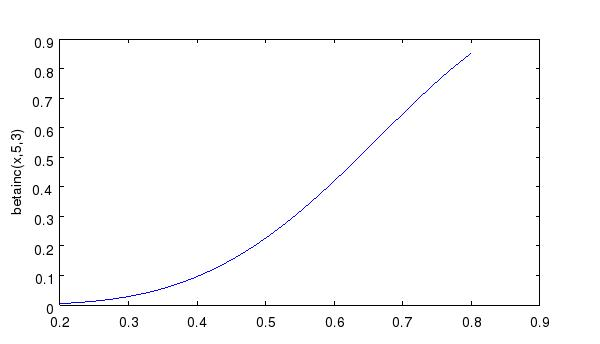
\includegraphics[width=8cm]{betainc1}}

